The next experiment we ran was to measure the amount of time it takes to run a procedure of 0-7 integer parameters. In addition, we measured the overhead for returning from a function call. 

Thus we implement each experiment as follows: 
\begin{verbatim}
void function(int v1, int v2, ... int vn){
  GET_HIGH(end);
}

unsigned long measure(){
  int v1 = 1;
  int v2 = 2;
  ...
  int vn = n;
  GET_HIGH(start);
  function(v1,v2, ... vn);
  return end - start;
}
\end{verbatim}

Note that, for standardization purposes, arguments are loaded into variables and passed to the function through these variables. This way, we know that the data is local, in cache and in the TLB, and computing the values to be passed to the function takes the same amount of time. This method is used in later experiments, where procedure call overhead affects the measurement, and must be subtracted.

We implement the return overhead experiment as follows:
\begin{verbatim}
void function() {
  GET_HIGH(start);
}

unsigned long measure() {
  function();
  GET_HIGH(end);
  return end - start;
}
\end{verbatim}

The overhead for a function call is plotted on the graph below.

\begin{figure}[h]
\centering
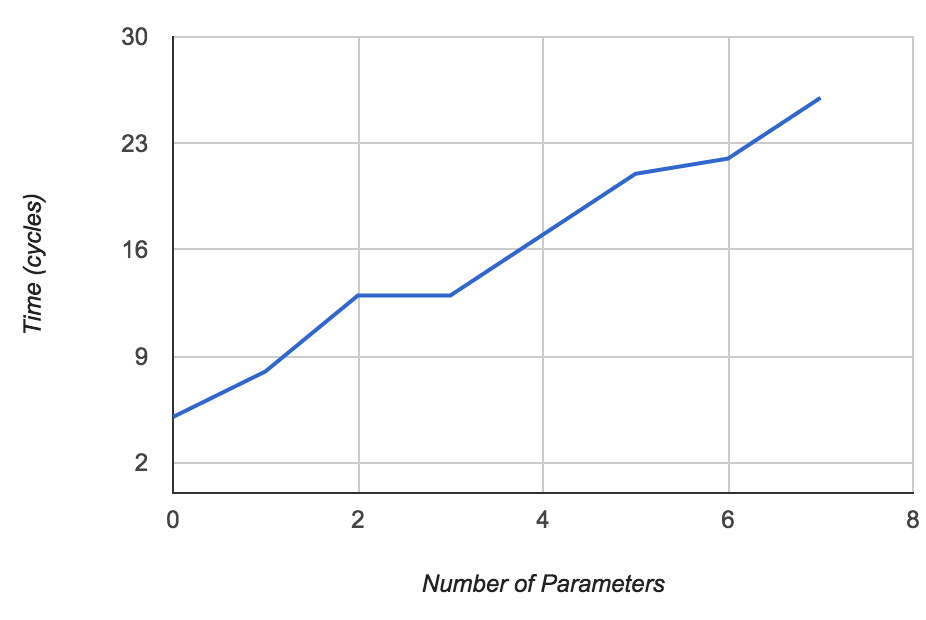
\includegraphics[scale=.5]{experiments/exp_1_2_fig.png}
\caption{Mean execution time vs number of parameters.  Overhead time included for comparison.  The standard deviation for all experiments was under 1 ns}
\end{figure}

There was a ~15 cycle overhead for procedure calls over the do nothing overhead.  Thus we were pretty close in our expected additional overhead for procedure calls.  There is also a strong linear relationship between number of procedure arguments and the time taken.  By performing a linear regression we get 4.2 ns additional cost per argument or about 3  additional cycles per parameter.